% !Mode:: "TeX:UTF-8"
% 室内可见光通信介绍

\chapter{室内可见光通信介绍}\label{chap:VLC-system}
\section{引言}
可见光通信系统的基本特性,如白光LED的光源特性,可见光通信的信道模型等,是本文进行后续组网技术研究的重要基础。
而LED作为一种新型的照明和通信方式,其在光学特性,电学特性和热学特性等方面都与传统的照明方式有着诸多的不同。
在室内可见光通信系统中,电学特性的频率响应,光学特性中的光源分布则是系统需要考虑的重点因素。
本章中,将会首先介绍可见光通信与传统的室内光通信的差异性,突出可见光通信的技术特点,
其次,着重对可见光通信的信道模型进行分析,以便用于后续的理论分析中。
接着,本章还将介绍室内光源对人眼安全的影响,从而对可见光通信的光源布局提出要求。
最后,将会从本文研究的组网技术作为出发点,介绍传统的相关系统,如蜂窝移动通信系统,无线局域网系统中的组网技术,并考虑以LED灯组作为通信设施之后带来的系统组网的问题。

\section{室内可见光通信系统概况}\label{sec:VLC-background}
\subsection{可见光通信与传统室内光通信的比较}\label{sec:Visible-IR}
传统的室内光通信通常采用红外线,紫外线等电磁波进行数据传输。这类光通信的技术特点较为相似,这里主要以红外线为例进行阐述。
由于红外通信的性价比高,跨平台,点对点传输速度较快等特性,已经被广泛地应用于室内短距离通信系统中,尤其是众多的嵌入式系统。
但是,使用红外线进行通信的这类室内光通信技术都有着较为明显的技术缺陷,这些缺陷将会限制着这类光通信技术的可持续发展,本文总结出如下几点主要问题。

首先,红外线可以透过角膜被晶状体吸收,可以被眼中的虹膜和睫状体吸收,从而会造成对视网膜的损害\cite{SongZhengXun2008},而紫外线同样也会对眼角膜上皮产生一定的危害,
因此,这类的室内光通信技术采用的传输介质是不安全的,对人们的身体健康有着较大的影响,同时,这种不安全性,也导致信号的发送功率被要求限制在一定的范围之内,
影响了数据的高速传输。其次,由于室内红外通信技术被不断地应用于人们的日常生活中,使得该段频谱资源变得日益紧缺,从而不得不采取严格的管理控制,这也会导致红外通信等室内光通信技术的发展受限。
另外,由于红外通信的指向特征很强,一旦通信中有其他的物体接入,对数据的正常传输会产生重要的影响,甚至会直接中断数据传输,这也就意味着这类光通信技术对通信环境比较敏感\cite{kahn1997}。
最后,类似红外线的此类光通信技术采用电磁波作为通信媒介进行数据传输,这在一些特定的场合下是不能被应用的,比如说在医院,飞机机舱等,因此,这些领域的室内无线通信需要使用一种新型的无线通信技术来解决。

而可见光通信则为上述的一系列问题提供了一个良好的解决方案,由于可见光通信采用白光作为传输媒介,因此不会对人们的身体产生任何影响,
同时可以根据通信的要求灵活地调节灯组的发送功率,而不必担心其对人们身体的影响。同时,白光的频谱资源非常可观,在使用时也无需进行资源的申请,这也是保证室内高速数据传输的重要基础。
此外,可见光通信可以用于上述提及的医院,飞机等禁止电磁波的区域,因此其适用范围相对较广。但是,使用可见光通信同样也存在着一定的局限性。
如具有通信定向性的特征,当灯组和用户进行通信的过程中,如果遇到遮挡等障碍物,则会影响通信的正常进行。另外,由于传统的无线通信技术的信号能量衰减与距离的平方成正比,
而光通信的信号能量衰减与距离的四次方成正比,因此光通信的传输距离范围要更加短。此外,室内光通信还面临着受背景噪声的影响较为严重,检测方式过于单一等问题。

文献\cite{Mei2011}对使用红外光和白光进行光通信系统通信媒介时的系统技术特征进行了较好的对比,其对照结果如\autoref{tab:IR-Visible}所示:

\begin{table}[htbp]
    \caption{使用红外光和白光作为室内光通信媒介时的技术特征对比}
    \label{tab:IR-Visible}
    \centering
    \begin{tabular}{lll}
        \toprule
        媒介特性 & 红外光 & 白光\\
        \midrule
        信号光源 & 红外LED、红外LD & 白光LED \\
        工作波长 & 典型波长800-900nm & 380-780nm \\
        调制带宽 & 几十kHz-几百MHz (LED) 几十kHz-几百GHz (LD) & 几十kHz-几百MHz (LED) \\
        信道速率 & 理论速率100Mb/s,实现16Mb/s & 目前最高速率达806Mb/s \\
        室内布局 & 需要另架设红外通信光源和线路 & 简化室内线路布局 \\
        阴影效应 & 容易受到其他遮挡物影响 & 安放多个LED灯消除阴影效应 \\
        发射功率 & 需限制发射功率,通信距离受限 & 通常情况下无需限制 \\
        \bottomrule
    \end{tabular}
\end{table}

通过上表将常见的室内光通信方式和可见光通信放在一起对比可以发现,可见光通信在室内布局,阴影效应,频谱资源等方面均大大优于现有的室内通信技术,
同时可以被应用的场合也更加广泛。因此,可见光通信技术作为目前的蜂窝无线通信技术的一个重要的补充,在室内提供短距离的高速数据通信具有非常广阔的研究前景。


\subsection{可见光通信系统的链接方式}\label{sec:vlc-on-link-mode}
目前的室内无线通信系统的链接方式的划分主要根据两种标准\cite{WuXia2014},发射和接收的定向性,以及是否存在视距传输。对于第一个划分标准,这里的定向性对于发射端和接收端的意义是不一样的,对于发射端而言,是要求发射出的光束的发散角很小且光束近乎平行,而对于接收端来说,就是其接收视场角很小。
由上述假设的发射和接收端组成的系统的链路就是定向链路。但如果上述两个条件都不成立,那么该系统的链路就是非定向链路。如果上述的两个条件一个成立,另一个不成立,那么此时系统的链路就被称为混合链路。
而对于第二个划分标准,则是通过发射端和接收端之间是否存在视距链路来进行划分。如果接收端接收的光信号既包含视距空间直接传输过来的直射光信号,又包含通过屋内的发射体发射过来的反射光信号,那么该链路就可以被划分为视距链路。
而如果接收端接收到的光信号只包含发射过来的反射光信号,那么该链路就要被划分为非视距链路。

根据上述提及的两种链路划分标准,一共可以产生6种可能的链路情形,其示意图如\autoref{fig:vlc-on-link-mode}所示\cite{WuXia2014}:

\begin{figure}[htbp]
    \centering
	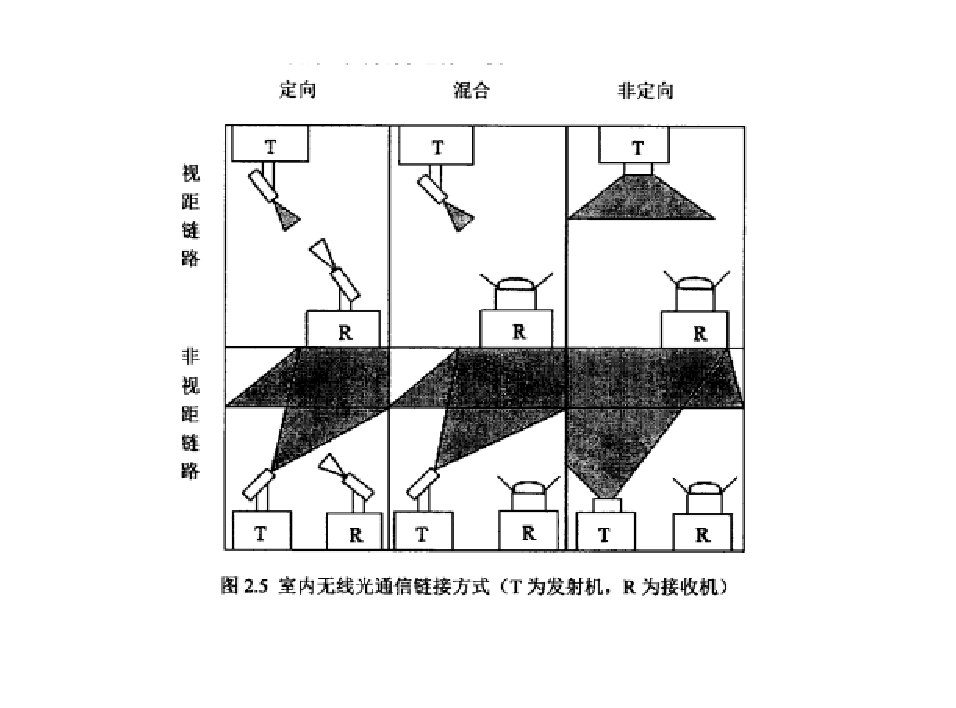
\includegraphics[width=0.8\textwidth]{figures/chapter-2/VlcOnLinkMode.eps}
	\caption{光通信链路划分标准}
	\label{fig:vlc-on-link-mode}
\end{figure}

对于使用可见光作为通信媒介的光通信来说,一般LED灯组都是安放在房间内的天花板上,而用户则处于房间内进行活动。
因此,一般意义上的可见光通信都采用的是视距链路方式。下面主要分析一下在视距链路下的三种不同的链路情况。

首先,考虑的是定向视距链路,使用这种链路类型的系统,为了保证通信的进行,要求发射端和接收端是对准的,由于发射端发出的光散射消耗的光功率较小,
同时接收端的视角又正好集中在发射方向的正对方向,因此这种情况下接收端获得的光接收功率会非常大,同时多径干扰也会非常的小。
但是采用这种方式,要求发射端和接收端要严格对准,一旦接收角度发生一定的变化,或者是链路收到其他障碍物的干扰,都会使得通信的质量大大下降。
同时,这种方式对于用户的移动性的支持也较差,所以它比较适合用于静态的点对点通信的场合中。

其次,可以考虑混合视距链路,对于该链路可以分为两种情况,一种是光发射机的发射角度很大,而光接收机的接收角度较小。另一种是光发射机的发射角度较小,而光接收机的接收角度很大。
对于第一种情况,虽然光发射机发射角度的增加使得接收端获得接收功率下降了,但是也同时提高了发射端光通信可以覆盖的范围,使得用户可以一定范围内运动下仍能保证和灯组进行通信。
而由于接收端的接收角度较小,使得接收端的多径干扰也大大降低,因此这是一种比较实用的光通信链路情形。而对于第二种情况,由于发送端的信号较为集中,而接收端的接收角度较大,这种方式下接收端产生的码间干扰和噪声干扰将会较大。

最后,对于非定向的视距链路而言,增大了发射角度和接收角度,同样这种方式可以对用户的移动性起到有利的影响,使得用户在较大的范围内可以获得灯组的发射信号。但是角度的增加也会带来多径干扰的增强,从而影响链路的通信质量。

在实际的光通信系统中,通常采用混合视距链路中的第一种情况或者是非定向的视距链路进行数据通信。由于在一般情况下,LED灯组的发射角度和灯组的类型有关系,在选定灯组后,该值也就确定了,所以可以研究接收端接收角度的变化对于系统产生的影响,
并选择合适的接收角度进行数据传输。

\subsection{可见光通信信道分析}\label{sec:vlc-channel}
由上述的分析可知,一般的可见光通信系统采用的是视距链路进行通信。对于视距链路下的通信信道,可以对其信道模型进行详细的分析。对于可见光通信系统而言,可以将其视为一个线性时不变系统\cite{DingJuPeng2005},该信道模型可以表示为:

\begin{equation}
    y(t) = \gamma \times (x(t) \otimes h(t)) + n(t)
    \label{equ:baseband-channel}
\end{equation}

其中,$y(t)$表示的是接收的电信号,$x(t)$表示的是发送的电信号,$h(t)$是系统的冲击响应,$\gamma$是接收端的检测灵敏度,$n(t)$为系统的加性高斯白噪声,$\otimes$表示卷积。

那么该信道的基本特征也就可以使用该系统的冲击响应$h(t)$来进行描述。这里,首先可以建立可见光通信系统通信时的几何模型,假设其通信时的平面位置图如\autoref{fig:vlc-ji-he}所示。

\begin{figure}[htbp]
    \centering
	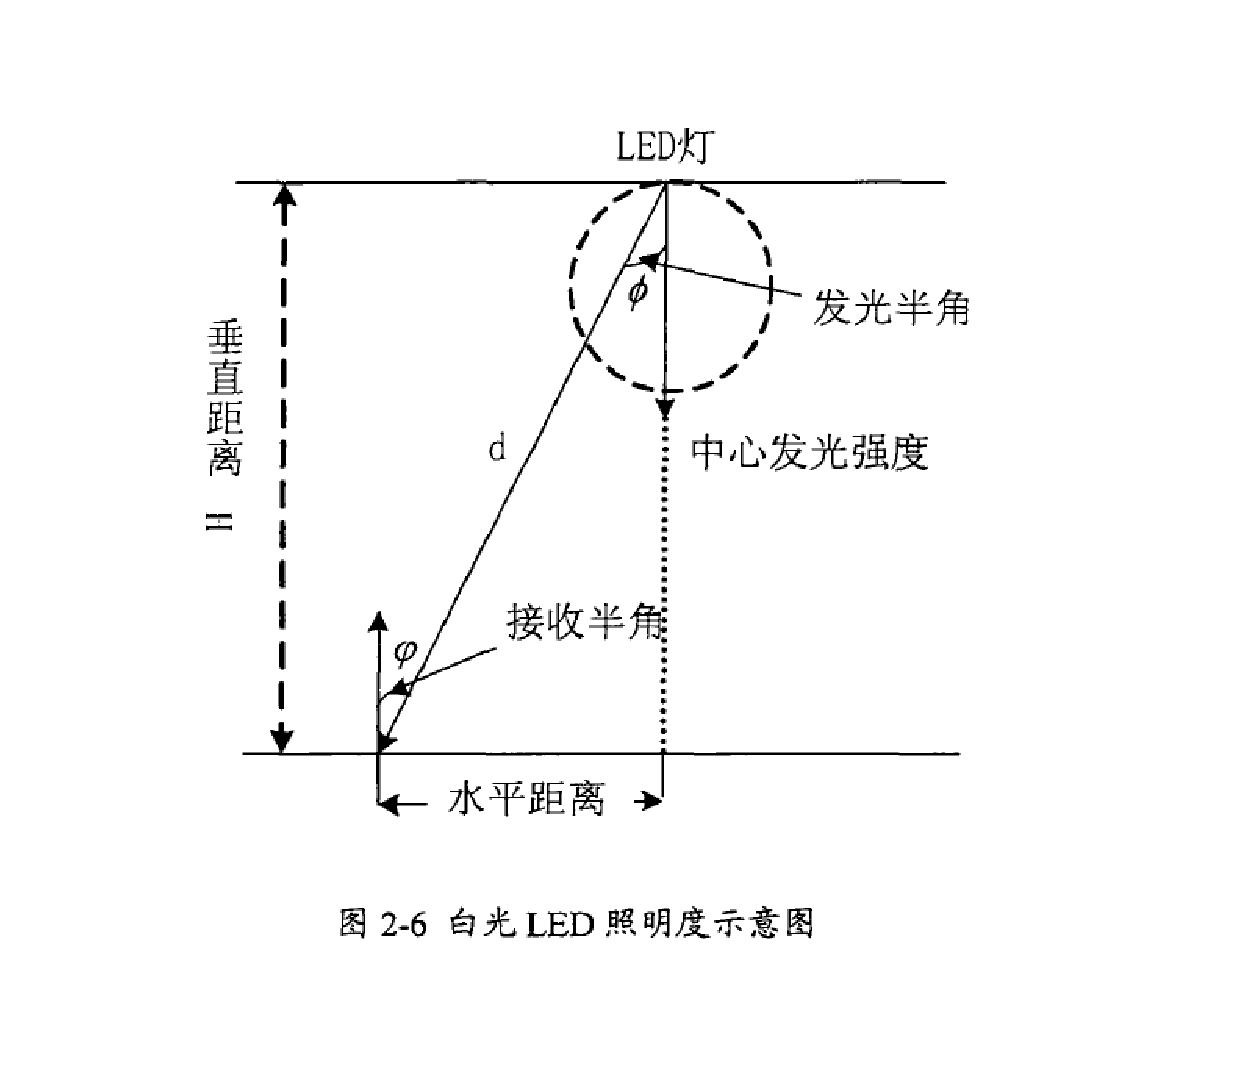
\includegraphics[width=0.8\textwidth]{figures/chapter-2/VlcJiHe.eps}
	\caption{光通信时的平面位置图}
	\label{fig:vlc-ji-he}
\end{figure}

假设发射端特征记为$S$,接收端特征记为$R$,环境特征记为$E$,当使用强度调制/直接检测的方式(Intensity Modulation / Direct Detection, IM/DD)进行通信时,系统的冲击响应可以表示为\cite{WuXia2014}:

\begin{equation}
    h_{E}(t;S,R) = \sum_{k=0}^\infty h_{E}^k(t;S,R)
\end{equation}

其中,$h_{E}^k(t)$表示的是在环境特征为E的条件下系统对第k条反射链路的冲击响应。假设系统发射端的光源采用朗伯辐射模型,如图\autoref{fig:lambo}所示\cite{ChenRan2013},图中的$n$表示白光光束的方向性,该值越大,说明光源的方向性也就越好。

\begin{figure}[htbp]
    \centering
	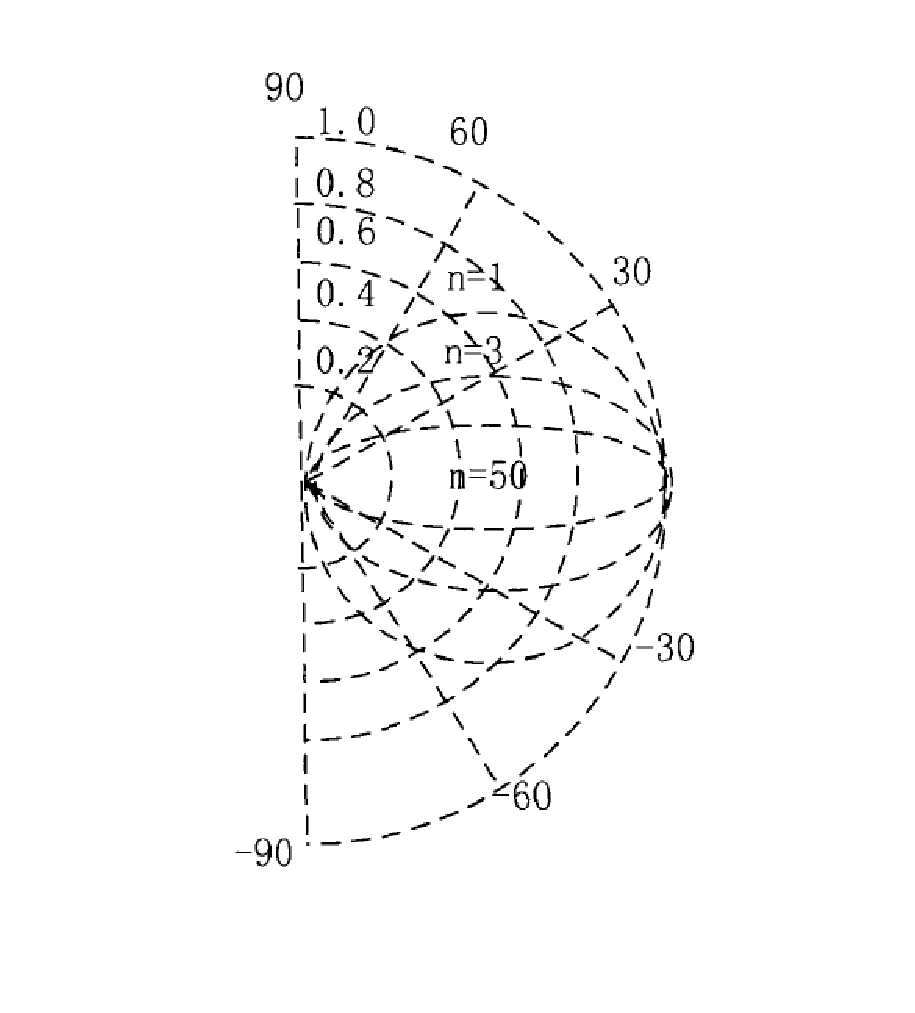
\includegraphics[width=0.7\textwidth]{figures/chapter-2/Lambo.eps}
	\caption{朗伯辐射模型}
	\label{fig:lambo}
\end{figure}

所以光源的辐射强度可以表示为:

\begin{equation}
    T(\phi) = \frac{m+1}{2\pi}\cos^m(\phi),\;\phi\in[-\frac{\pi}{2},\frac{\pi}{2}]
\end{equation}

其中,$m$为朗伯辐射系数,该值和光源的半功率强度有关,$\phi$为接收的角度值。

该模型下系统的发射端特征可以由光源位置$r_{S}$,单位方向向量$n_{S}$和上述的朗伯辐射系数这三元组来确定,即

\begin{equation}
    S=\left\{r_{S},n_{S},m\right\}
\end{equation}

同样,接收端的特征也可以用接收端位置向量$r_{R}$,单位方向向量$n_{R}$,接收端面积$A_{R}$和接收视场角$FOV$这四元组来进行表示

\begin{equation}
    S=\left\{r_{R},n_{R},A_{R},FOV\right\}
\end{equation}

在计算系统的脉冲响应时,通常先观察零次反射的响应函数,即从发射端通过直达径达到接收端时的响应,表示如下\cite{WuXia2014}

\begin{equation}
    h_{E}^0(t;S,R)=V(E)T(\varphi)(\frac{A_{r}g_{a}(\theta)}{D^2})\delta(t-\frac{D}{c})
\end{equation}

其中$V(E)$表示的在环境特征$E$的条件下的可视函数,如果直达路径上是没有遮挡的,那么该值为1,否则该值为0。$T(\varphi)$是指采用的辐射模型,
$A_{r}$是光接收面积,$D$是源端和接收端之间的距离, $g_{a}(theta)$是接收器的增益函数,可以表示为

\begin{equation}
    g_{a}(\theta)=
    \begin{cases}
        1,  & \theta\le\psi_{c} \\
        0,  & \theta>\psi_{c}
    \end{cases}
\end{equation}

其中,$\theta$为接收端的入射角,$\Psi_{c}$为接收端的视场角。

当获得了$k$-1次反射响应函数之后,就可以通过迭代的方式求出第$k$次反射的响应函数[36]:

\begin{equation}
    h_{E}^k(t;S,R)=\int_{S} \rho_{r}h_{E}^{k-1}(t;\{r,n,1\},R)\otimes h_{E}^0(t;S,\{r,n,\frac{\pi}{2}, \, dr^2\})
\end{equation}

上述意味着在环境特征为$E$的条件下,对于接收端的表面进行积分。$r$是$S$中的微反射体的位置向量,$\rho_{r}$是$r$处微反射面的发射系数,$n$是$r$处微反射面的单位法向量。

这样通过式(2-5)和式(2-7),可以得到接收端的任意第k次的发射响应函数。
而在实际情况下,并不需要考虑无穷次的发射链路的冲击响应,因为随着反射次数的增加,对应的冲击响应的能量值也越来越小,
所以在计算总的冲击响应时,只需要考虑前M次的反射的冲击响应即可,所以总的冲击响应的表达式可以如下表示

\begin{equation}
    h_{E}(t;S,R)\approx \sum_{k=0}^M h_{E}^k(t;S,R)
\end{equation}

一般情况下,M取3到10即可表现出整体的冲击响应\cite{DingJuPeng2005}。因此,通过上式,就可以求出室内可见光通信系统中的总的冲击响应表达式。

在室内可见光通信系统中,若只考虑直达路径,接收端的光接收功率可以表示为

\begin{equation}
    P_{r}=H_{E}(0;S,R)P_{t}
\end{equation}

其中,$P_{t}$为发射端的光发射功率,$H_{E}(0;S,R)$为信道的直流增益。该值则可以通过系统的冲击响应积分计算得到,即

\begin{equation}
    H_{E}(0;S,R)=\int_{-infty}^{+infty} h_{E}(0;S,R)\, dt
\end{equation}

将上述的式(2-8)代入式(2-10)后,可以得到直流增益的表达式为

\begin{equation}
    H_{E}(0;S,R)=
    \begin{cases}
        \frac{(m+1)A}{2\pi D_{d}^2}\cos^m(\phi)T_{s}(\psi)g(\psi)\cos(\psi),  & 0\le\psi\le\psi_{c} \\
        0,  & \psi>\psi_{c}
    \end{cases}
\end{equation}

其中,$\phi$是发射信号出射角,$\psi$是接收信号入射角,$m$是朗伯系数,$A$是接收端的探测面积,$D_{d}$是灯组和用户之间的距离,$T_{s}(\psi)$是光滤波器的增益值, $\psi_{c}$是接收端的视场角。$g(\psi)$是光接收器的增益,可以表示为

\begin{equation}
    g(\psi)=
    \begin{cases}
        \frac{n^2}{\sin^2\psi},  & 0\le\psi\le\psi_{c} \\
        0,  & \psi>\psi_{c}
    \end{cases}
\end{equation}

另外,还需要考虑此时的系统接收信噪比。假设发射端发射的信号为 ,接收端收到的电信号功率可以表示为

\begin{equation}
    S=\gamma^2P_{rSig}^2
\end{equation}

其中$\gamma$表示的是接收端的光电转换效率,而$P_{rSig}$则是在单位时间内接收到的信号的功率,可以表示为

\begin{equation}
    P_{rSig}=\int_{0}^{T} h(t) \otimes x(t)\, dt
\end{equation}

而在室内光通信条件下,接收端的噪声主要由三部分组成,即为散粒噪声,热噪声和码间干扰噪声\cite{WuXia2014},所以总的系统噪声可以表示成

\begin{equation}
    N=\sigma_{shot}^2+\sigma_{thermal}^{2}+\gamma^2P_{rISI}^2
\end{equation}

其中各部分的噪声也可以分别表示为\cite{KomineT2004}:

\begin{equation}
    \sigma_{shot}^2=2q\gamma(P_{rSig}+P_{rISI})B+2qI_{bg}I_{2}B
\end{equation}

\begin{equation}
    \sigma_{thermal}^2=\frac{8\pi kT_{k}}{G}\eta AI_{2}B^2+\frac{16\pi^2kT_{k}\Gamma}{g_{m}}\eta^2A^2I_{3}B^3
\end{equation}

\begin{equation}
    P_{rISI}=\int_{T}^{\infty}h(t) \otimes x(t)\, dt
\end{equation}

其中,$q$为电子的带电量,$B$为接收电路的等效噪声带宽,$k$为玻尔兹曼常数,$T_{k}$为绝对温度,$\eta$指探测器单位面积上的电容,$I_{bg}$为背景电流,$I_{2}$为噪声带宽因子,$G$为开环电压增益,$\Gamma$为FET噪声因子,$g_{m}$ 为FET的跨导,$I_{3}$为常数。

因此,接收端的接收信噪比SNR也就可以通过下式计算得到

\begin{equation}
    SNR=\frac{P_{rSig}}{N}
\end{equation}

根据上述理论分析,可以计算出系统接收的信噪比。同时,上述的分析也展示了影响接收端信噪比的两个重要方面。首先,在上述计算信噪比的过程中,采用的是总的系统冲击响应,
但是在实际的过程中,根据文献\cite{Yu2009}的描述,在室内可见光通信系统中,通过墙面等反射体的发射到达接收平面的信号能量要远小于通过直达径到达的信号能量,因此在实际仿真中计算接收端的信噪比时,
在信号功率的计算方面,可以只计算直达径获得的信号能量,忽略通过发射到达接收端的信号能量。其次,由于信噪比中的噪声除了受系统的热噪声等不可抗拒因素影响以外,还很大程度上取决于系统接收端的码间干扰。
而接收端码间干扰的形成则是由于发送端的信号经过多个不同的光路径达到接收端。这里的发送端的光信号可能既来自目的灯组,也来自目的灯组以外而定其他不同的光源。
所以,当我们在设置室内的LED灯组布局时,既要考虑到通过增加LED灯组的个数,减小接收平面的"阴影"区域,同时还需要注意多个LED灯组的重叠覆盖导致的用户接收端的多径效应\cite{DingDQ2006}。

\section{通信系统组网技术研究}\label{sec:network-tech-researh}
\subsection{相关系统的组网方案}
在移动通信领域,对于组网技术的研究也一直是一个热门的问题。对于移动通信网的组网的定义,一般是以增加系统的效益作为目标,采用各种通信技术和设备来有效地组织、管理和调度网络。

在目前推出的准4G标准LTE中,使用了六类组网技术来克服系统对于上下行组网时遇到的挑战,文献\cite{LiuXiaoFeng2010}对LTE系统中的组网技术进行了较为完善的总结,
其将LTE中的组网技术归纳为以下6点:时域与频域调度、跳频、码分复用、空间波束赋形、功率控制和接收机算法增强。其中,时域与频域调度是为了抑制小区内部的干扰,采用对时域和频域资源的合理调度,
达到多用户的无干扰数据传输。调频技术则是在上述的数据传输中,对于同一用户在不同的时刻采用不同的频率进行传输。LTE中的码分复用是体现在两个方面,一个是加扰,另一个是扩频,
加扰是使用一定的随机序列对小区发送的数据进行扰乱,从而使得干扰随机化,来抑制小区间的干扰。而扩频则是利用无关的码来对被传输信号进行频谱扩展,从而有效抑制干扰。空间波束赋形则是通过对多天线阵列的控制,
使得发送出去的信号呈现一定的方向性,从而可以根据用户的位置,发射信号时选择正确的方向,并抑制用户之间的干扰。由于LTE系统使用的是同频覆盖,因此功率控制的目的是指通过对系统中的资源进行合理的管理,
从而协调好多个小区之间的动作,从而避免产生严重的小区间干扰。接收机算法增强也是指干扰删除,包括基于多天线的空间干扰压制技术和基于干扰重构的干扰消除技术。上述组网技术保证了在LTE系统中对基站间的相互干扰取得有效地控制,
从而获得整个网络的更高的吞吐量。

而作为室内无线通信最常使用的无线局域网技术,其组网方式通常可以分为两种类型,对等网络和基础结构网络\cite{LiHaoLing2008ap}。其中对等网络,是指由一组具有无线接口的计算机组成的网络,网络中的任意两台机器都可以进行直接通信。
而在基础结构网络中,使用了无线接入点将无线局域网和有线网连接起来,在无线局域网中,各节点通过接入点进行相互通信。对于广泛使用的基础结构网络中,又分别提出了胖接入点(Fat AP)技术和瘦接入点(Fit AP)技术\cite{LiHaoLing2008ap},并根据实际的场景进行定制。胖接入点技术将无线局域网中的物理层,数据加密,用户认证,网络管理,漫游技术和应用层技术结合起来,
使得每个胖接入点都可以成为一个独立和有线网连接的个体。但是胖接入点只能进行单独配置,且所有的软件都要保存在接入点上,在大型网络下对于接入点的管理和维护工作量大。
因此,瘦接入点技术被提出。瘦接入点只完成无线局域网中的物理层的工作,而其他的功能,如用户认证,安全管理,网络管理和应用层功能都被上移到接入控制器(AC)上进行。
这样的好处就是在进行大规模组网的时候,只需要对接入控制器进行配置,部署便捷,同时此类系统还可以支持快速切换,并可以进行有效的网络安全管理和控制。

\subsection{室内光通信系统组网的问题}
上述提及的是移动蜂窝网和局域网中常用的组网方式,而在室内可见光通信系统中,考虑到可见光通信的技术特点和典型的组网架构,组网中的关键技术主要包括可见光光源布局研究,可见光网络切换技术,
可见光网络接入控制技术,系统级的资源分配方案等一系列的内容\cite{LiuYang2014}。

其中,可见光的光源布局是指采用合理的光源布局,来满足可见光通信系统的照明和照明的需求。在常见的光通信应用场景中,通常使用多个灯组进行室内有效地覆盖,作为通信设备使用的灯组,
其布局情况必定对整个系统的性能有着重要的影响。对于光源的布局设计,需要考虑到房间的大小,灯组的选择,直射距离等信息,从而对LED间隔的大小,排列和位置,LED灯组的个数等信息进行合理的设计,从而保证系统的通信性能。

可见光网络切换技术则是为了支持室内用户的移动性,当用户在室内随意走动时,仍能保证用户和灯组之前的可靠链路通信。这是因为光通信的一个显著特点就是信号的衰减较快,因此每个灯组的覆盖面积较小,
当用户进行了移动后,很有可能就会从一个灯组的覆盖区域移动到另外一个灯组的覆盖区域,所以,灯组之间的垂直或是水平切换策略就显得特别重要。类似于蜂窝通信系统,在可见光通信系统中一般会对某用户的当前服务灯组的信号质量进行跟踪,
当发现当前的服务灯组的信号差到一定的程度时,就需要寻找新的可接入灯组并选择合适的接入方式进行接入。

可见光网络接入控制技术则是为了在有下行干扰的条件下,进行上行接入的控制技术。由于在进行灯组组网时,接收平面是很多地方是多个灯组的重叠覆盖区域,因此,当用户处于这些位置时,就会存在较为严重的相邻灯组下行干扰,
如果用户上行传输仍然是采用光通信的话,就必须使用某种接入控制技术,例如采用基于角度感知的定向接入协议,来保证干扰下用户上行通信的进行。

系统级的资源分配方案则是针对于当前的灯组布局和用户的情况,采用合适的灯组调度策略,减小系统中用户之前的干扰,并实现系统吞吐量的最大化。
在不同的光通信系统中,灯组的控制方式也可以是不一样的,就如上述的局域网系统而言,如果所有的灯组的控制功能如用户鉴权,加密,漫游控制等全部由连接各灯组的控制中心负责,
各个灯组可以看作是一个单纯负责物理层通信的实体,那么这种控制方式可以被称为分布式灯组控制,而如果所有的灯组都具有对其覆盖范围内的用户具有控制功能,每个灯组可以进行独立的配置,
那么这种控制方式可以称为独立式灯组控制。针对这两种情况,可以分别进行研究,讨论需要采用何种的调度策略进行系统资源的分配,从而保证多用户的光通信系统可以获得较大的系统容量。

上述这些组网技术将会保证可见光通信系统可以更加高效地使用资源,更加灵活地配置和管理网络,对光通信系统的实际的运行具有重要的意义。在本文的后续章节中,鉴于本文的承载量,本文将会对上述组网技术中的部分内容进行研究和分析。

\section{本章小结}
本章主要介绍了可见光通信系统的基础理论,为之后章节的具体分析奠定了理论基础。
首先,介绍了室内可见光通信和传统的室内光通信(以红外通信为例)的区别,并通过比较可以了解到室内可见光通信在频谱资源,安全性,适用范围等方面的显著优势。
这也是可见光通信将会代替目前的室内光通信技术的一个重要依据。
接着,本章介绍了室内光通信的链路方式的划分标准,并指出了常见的可见光通信的链路方式,
以此为基础,本章介绍了可见光通信的信道模型,并对接收端的信噪比等典型参数进行了理论分析。
最后,本章还重点对于研究的组网领域进行了介绍。主要介绍了常见的通信系统,如移动蜂窝系统和室内局域网系统中目前常用的组网技术,
同时介绍了可见光通信系统在组网方面需要解决的关键技术问题,为后续的本文研究指明了研究的方向。
